\section{Appendix}

The survey of the user study contains the following elements:
\begin{enumerate}
	\item Introduction \& consent form
	\item \textit{Scenario 1}: Social media administrator and manual offensive language detection
	\item \textit{Tweet block 1}: 15 Tweets for classification, on individual pages (no system)
	\item \textit{Scenario 2}: Introduction to automatic decision system supporting the task
	\item \textit{Tweet block 2}: Repetition of 15 Tweets for classification, on individual pages (with system)
	\item Perceived understanding \& trust questionnaire
	\item Demographics
	\item Outroduction \& crowdsourcing completion codes
\end{enumerate}
This section lists the scenario formulation used in the study, as well as the questionnaires for perceived understanding, trust, and demographics.

\subsection{Scenario 1: Scene}
For answering the upcoming questions, \textbf{please read the following scenario carefully} before continuing to the next page. \medskip \newline
Imagine you work for a youth TV channel that targets \textbf{people at the age of 15-20 years}.
You are the company's \textbf{social media administrator}.\newline 
Your responsibilities are:
\begin{enumerate}
	\item Upload new content on various platforms, e.g. Facebook, Twitter, Instagram
	\item Answer messages
	\item Moderate discussions and comments
	\item Ensure that the language of comments is appropriate: delete comments with offensive language and block users
\end{enumerate}
To support your work, you are given the ``\textbf{Administration Tool}". The ``Administration Tool" is a program that notifies you of new messages, lets you upload content to your social media channels, and alerts you in case of an inappropriate comment.
\begin{figure} [H]
	\centering
	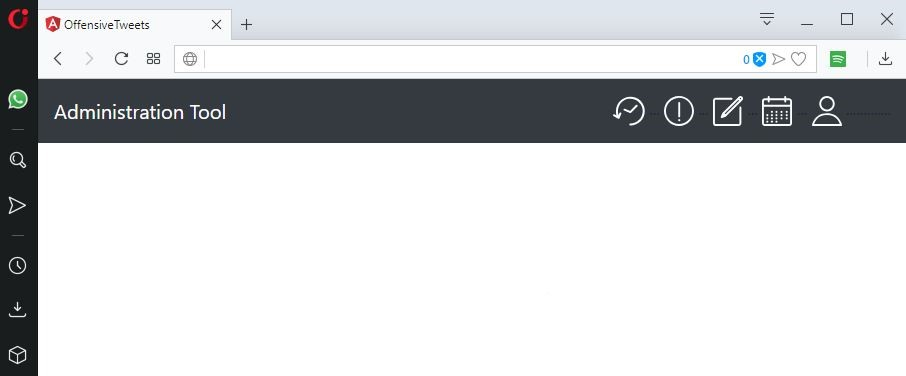
\includegraphics[width=0.8\textwidth]{img/administrationTool.JPG}
	\label{fig:app_admin_tool}
\end{figure}
\noindent Today, your manager asked you to review Tweets that may or may not contain \textbf{inappropriate, offensive language}.\newline 
To protect the \textbf{children and young adults} visiting your page, your company has strict rules on what ``offensive" means:\newline 
\begin{enumerate}
\item Containing \textbf{hateful} language: any comment that disparages a person or a group on the basis of some characteristic such as race, colour, ethnicity, gender, sexual orientation, nationality, and religion
\item Containing \textbf{pornographic} language: explicit sexual subject matter for the purposes of sexual arousal and erotic satisfaction
\item Containing \textbf{vulgar} language: coarse and rude expressions, which include explicit and offensive reference to sex or bodily functions
\item Not only single words can be offensive, but also the \textbf{meaning} of a text. A text can be offensive without explicitly mentioning offensive words.
\end{enumerate}
On the next page, you will see 15 screenshots of the ``Administration Tool".\newline
\textbf{Please classify the Tweets on the screenshots using the above-mentioned guidelines into ``offensive" and ``not offensive".}\newline
The Tweets are taken directly from social media and may therefore include \textbf{typos, grammatical mistakes, and slang words}.\newline



\subsection{Tweet Block 1: Without System}
An exemplary screenshot of a survey page in block 1:
\begin{figure} [H]
	\centering
	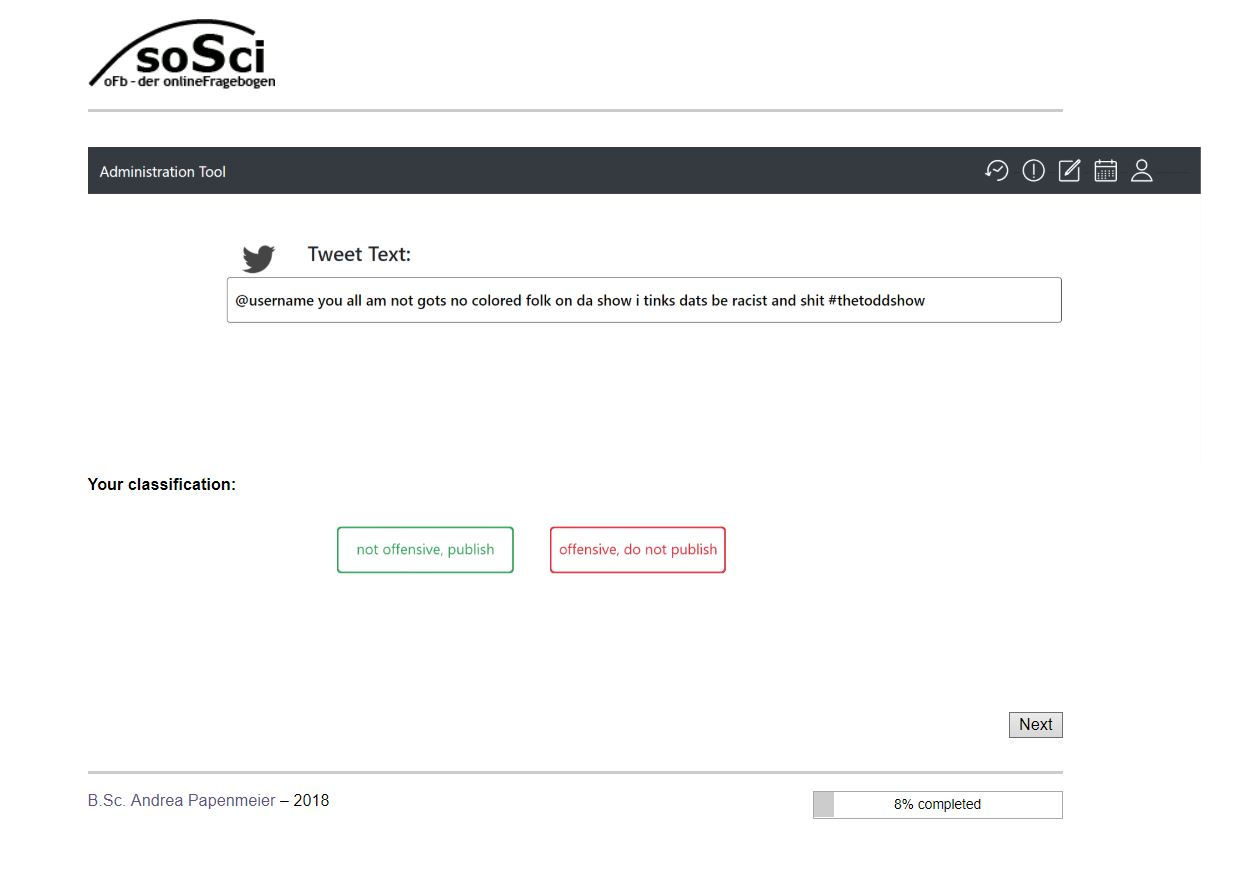
\includegraphics[width=0.8\textwidth]{img/app_screenshot_no_sys.JPG}
	\label{fig:app_block1}
\end{figure}



\subsection{Scenario 2: Task}
For answering the upcoming questions, \textbf{please read the following scenario carefully} before continuing to the next page. \medskip \newline
The ``Administration Tool" team has developed a system that automatically detects offensive Tweets.
The automatic detection system shows the result of its computation as follows:
\begin{figure} [H]
	\centering
	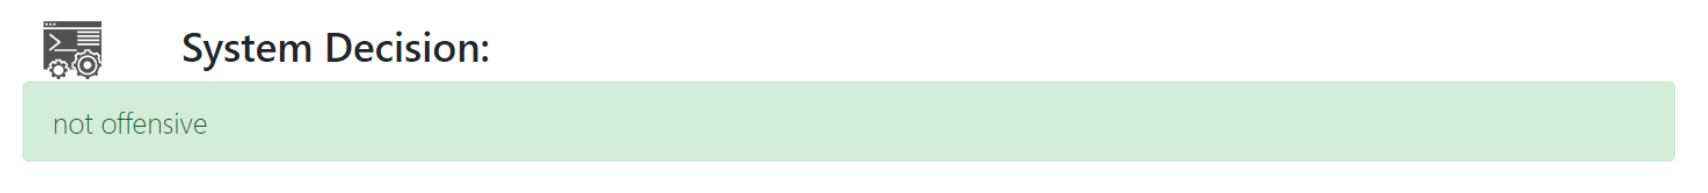
\includegraphics[width=0.8\textwidth]{img/example_decNotOffensive.JPG}
	\label{fig:app_decision_non_offensive}
\end{figure}
and 
\begin{figure} [H]
	\centering
	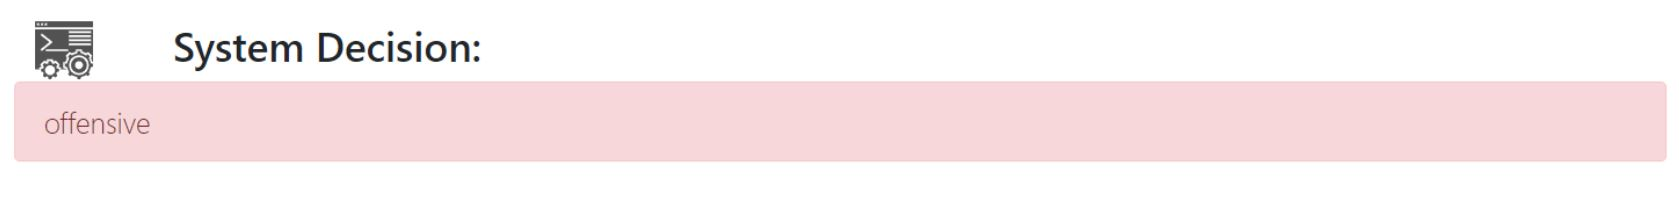
\includegraphics[width=0.8\textwidth]{img/example_decOffensive.JPG}
	\label{fig:app_decision_offensive}
\end{figure}
\noindent On the next page, you will see 15 Tweets very similarly to the ones before. This time, the automatic detection system assists you in your task.\newline
\textbf{Please classify the Tweets on the screenshots into ``offensive" and ``not offensive"}.



\subsection{Tweet Block 2: With System}
An exemplary screenshot of a survey page in block 2:
\begin{figure} [H]
	\centering
	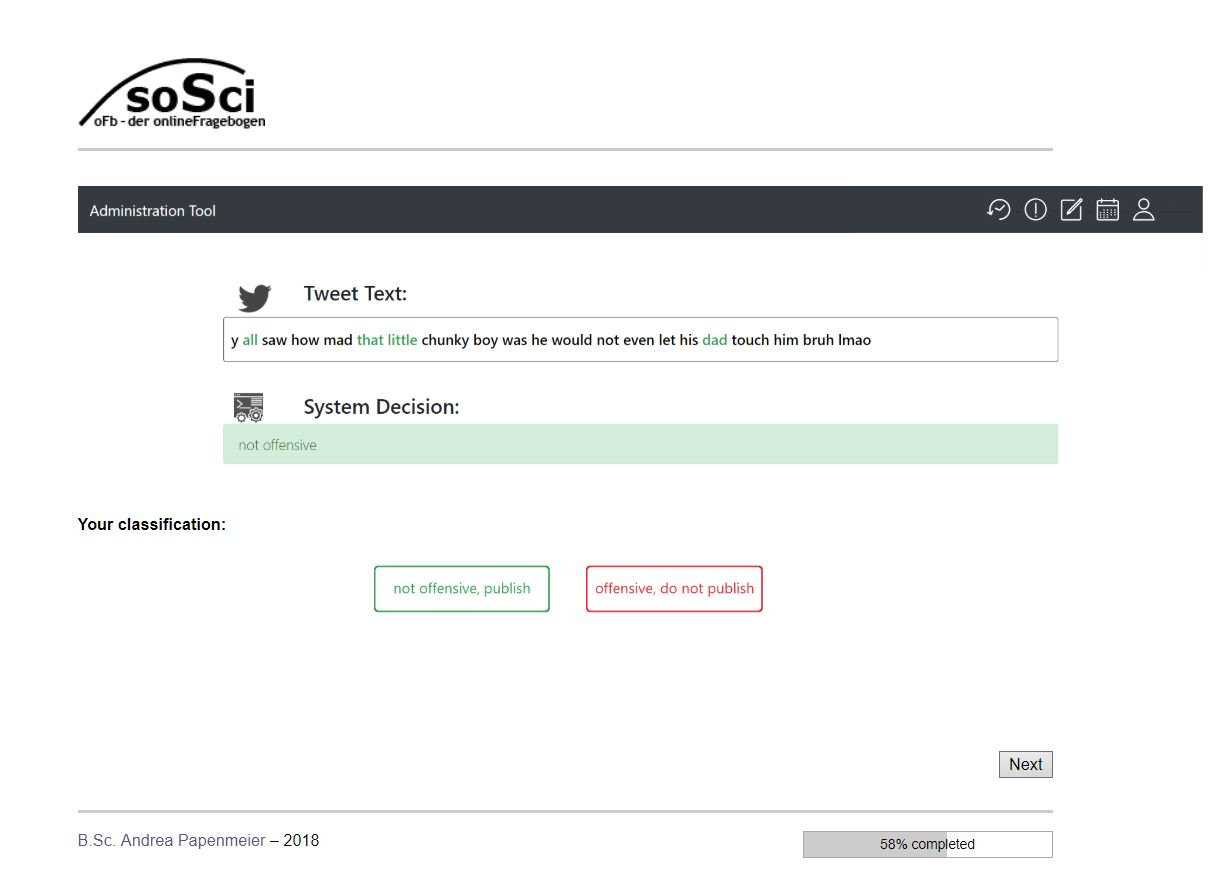
\includegraphics[width=0.8\textwidth]{img/app_screenshot_sys.JPG}
	\label{fig:app_block2}
\end{figure}



\subsection{Questionnaire Perceived Understanding}
\textbf{Please evaluate how confident you are in your understanding of the automatic classification system.}
\begin{enumerate}
	\item The decision (``offensive", ``not offensive") the system made for a single Tweet	
	\item The reason why the system made the decision	
	\item The important factors that contributed to the decision
\end{enumerate}
Evaluation on a 5-points Likert scale with labelling of the extrema: ``not confident that I understand" (left) and ``totally confident that I understand" (right)



\subsection{Questionnaire Trust}
\textbf{Please indicate your level of agreement with the following statements.}
\begin{enumerate}
	\item The system is capable of interpreting situations correctly.
	\item The system state was always clear to me.
	\item I already know similar systems.
	\item The system's developers are trustworthy.
	\item One should be careful with unfamiliar automated systems.
	\item The system works reliably.
	\item The system reacts unpredictably.
	\item The system's developers take my well-being seriously.
	\item I trust the system.
	\item A system malfunction is likely.
	\item I was able to understand why things happened.
	\item Please tick ``strongly disagree" to show that you are not a robot.
	\item I rather trust a system than I mistrust it.
	\item The system is capable of taking over complicated tasks.
	\item I can rely on the system.
	\item The system might make sporadic errors.
	\item It's difficult to identify what the system will do next.
	\item I have already used similar systems.
	\item Automated systems generally work well.
	\item I am confident about the system's capabilities.
\end{enumerate}
Evaluation on a 5-points Likert scale with labelling of each point: ``strongly disagree", ``rather disagree", ``neither disagree nor agree", ``rather agree", ``strongly agree".



\subsection{Demographics}
\textbf{What is your age?}
\begin{itemize}
	\item 18-30 
	\item 31-40
	\item 41-50
	\item 50+
\end{itemize}
\textbf{With which gender do you identify most?}
\begin{itemize}
	\item Male
	\item Female
	\item Inter / diverse
\end{itemize}
\textbf{In which culture were you primarily raised?}
\begin{itemize}
	\item Caucasian (e.g. European, North American, Central Asian)
	\item Latino / Hispanic
	\item Middle Eastern
	\item African
	\item Caribbean
	\item South Asian
	\item East Asian
\end{itemize}
\textbf{In which country did you spend most of your life time?}\newline
(Dropdown menu)\medskip \newline

\noindent \textbf{How do you self-assess your level of English language?}\newline
We use the Common European Framework of Reference for Languages (CEFR) scale:
\begin{itemize}
	\item C2	Proficient
	\item C1	Advanced
	\item B2	Upper-intermediate
	\item B1	Intermediate
	\item A2	Pre-intermediate
	\item A1	Elementary
	\item A0-A1	Beginner
\end{itemize}
